\usetikzlibrary{plotmarks}

\begin{figure}[htbp]
\centering
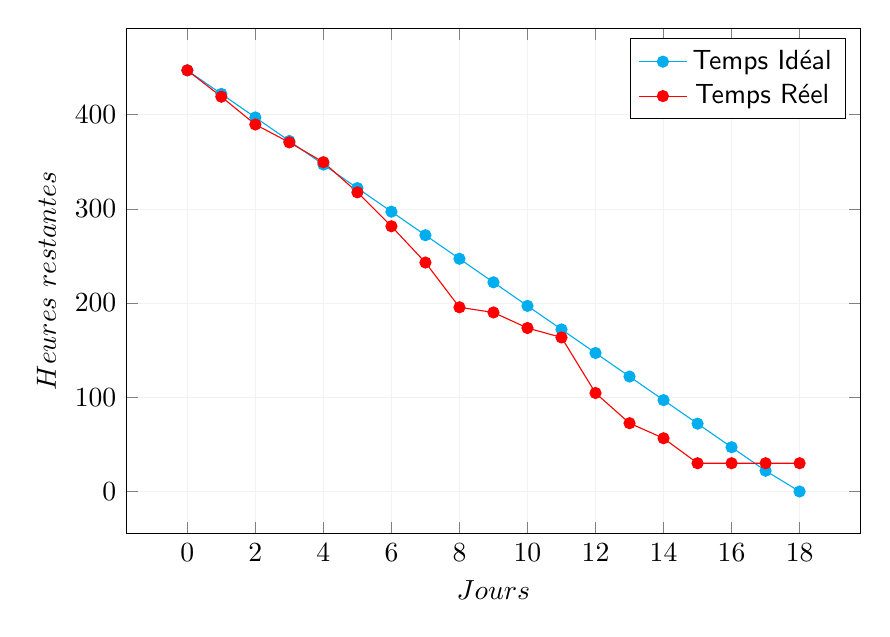
\begin{tikzpicture}[y=.2cm, x=.7cm,font=\sffamily]
\begin{axis}[
xlabel=$Jours$,
ylabel=$Heures\ restantes$,
grid=both,
grid style={line width=.1pt, draw=gray!10},
width=0.9\textwidth,
height=8cm,
%major grid style={line width=.2pt,draw=gray!50},
]
      \addplot[mark=*,cyan] plot coordinates {%
              (0, 447)
              (1, 422)
              (2, 397)
              (3, 372)
              (4, 347)
              (5, 322)
              (6, 297)
              (7, 272)
              (8, 247)
              (9, 222)
              (10, 197)
              (11, 172)
              (12, 147)
              (13, 122)
              (14, 97)
              (15, 72)
              (16, 47)
              (17, 22)
              (18, 0)
    };
    \addlegendentry{Temps Idéal}

    \addplot[mark=*,red] plot coordinates {%
        (0, 447)
        (1, 419)
        (2, 389.5)
        (3, 370.5)
        (4, 349.5)
        (5, 317.5)
        (6, 281.5)
        (7, 243)
        (8, 195.5)
        (9, 190)
        (10, 173.5)
        (11, 163.5)
        (12, 104.5)
        (13, 72.5)
        (14, 56.5)
        (15, 30)
        (16, 30)
        (17, 30)
        (18, 30)
    };
    \addlegendentry{Temps Réel}
\end{axis}
\end{tikzpicture}
\caption{Graphique d'avancement - Itération 2}
\label{fig:sprint2-burndown}
\end{figure}
